\documentclass{article}
\usepackage[utf8]{inputenc}
\usepackage[spanish]{babel}
\usepackage{listings}
\usepackage{graphicx}
\graphicspath{ {./images/} }
\usepackage{cite}

\begin{document}

\begin{titlepage}
    \begin{center}
        \vspace*{1cm}
            
        \Huge
        \textbf{Taller Memoria}
            
        \vspace{0.5cm}
        \LARGE
        Informática 2
            
        \vspace{1.5cm}
            
        \textbf{John Jairo Uribe Giraldo}
        
            
        \vfill
            
        \vspace{0.8cm}
            
        \Large
        Despartamento de Ingeniería Electrónica y Telecomunicaciones\\
        Universidad de Antioquia\\
        Medellín\\
        Septiembre de 2020
            
    \end{center}
\end{titlepage}

\tableofcontents
\newpage

\section{Sección introductoria}
Esta es el primer taller de la materia de Informática 2, en el se dará respuesta a 4 preguntas planteadas, la primera acerca de la memoria del computador; la segunda pregunta se refiere a los tipos de memoria conocidos y una breve descripción; la tercera a la manera como se gestiona la memoria y por último acerca de la velocidad de los diferentes tipos de memoria.

También tiene como objeto introducirnos en el manejo de aplicaciones tales como: Overleaf (para aprender a hacer texto a través de comandos), Git (aplicación para aprender a crear repositorios) y la plataforma Github (donde empezaremos a montar los repositorios.
\newpage
\section{Sección de contenido} \label{contenido}

\section*{\subsection{Defina que es la memoria del computador:}}
Es similar al cerebro humano; es el componente del computador  que apoya los procesos de almacenamiento de información tales como datos e instrucciones,   incluso permite ejecutar procesos temporales de los programas.Un computador sin memoria, no podria arrancar. La memoria esta dividida en un gran número de pequeñas partes llamadas celdas. Cada ubicación o celda tiene una única dirección, la cual varia desde cero hasta el tamaño de la memoria menos uno. Por ejemplo si el computador tiene 64 mil palabras, entonces la unidad de memoria tiene 64 * 1024 = 65536 ubicaciones de memoria. La dirección de estas ubicaciones varia desde cero hasta 65535.

\begin{figure}[h]
\caption{Computer Memory}
\centering
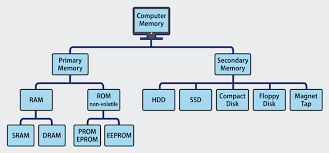
\includegraphics[width=0.5\textwidth]{memoria}
\end{figure}

\subsection{Mencione los tipos de memoria que conoce y haga una pequeña descripción de cada tipo:}

\subsubsection{Memoria RAM(Random Access Memory):}
 Memoria de Acceso Aleatorio, como su nombre lo indica permite almacenar informacion de manera temporal, es decir que cuando se reinicia el pc o hay ausencia de fluido eléctrico, lo que hay en la memoria ram se borra. 
 El tiempo de acceso en la RAM es independiente de la dirección, es decir, cada ubicación de almacenamiento dentro de la memoria es tan fácil de alcanzar como otras ubicaciones y requiere la misma cantidad de tiempo.
 Existen dos clases de memoria ram:
 \begin{itemize}
  \item SRAM, RAM Estática
  \item DRAM, RAM Dinámica
\end{itemize}

\begin{figure}[h]
\caption{Memoria RAM}
\centering
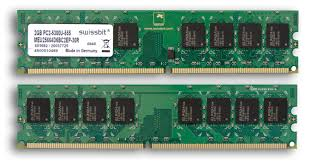
\includegraphics[width=0.5\textwidth]{RAM}
\end{figure}
\newpage
\subsubsection{Memoria ROM (Ready Only Memory):}
 Memoria de solo lectura, almacena informacion importante del sistema y de algunos programas. La información se almacena permanentemente en estas memorias durante su fabricación.
 La ROM almacena las instrucciones que son requeridas para iniciar el computador, esta operación es referida al bootstrap. La ROM no es usada solo en computadores, también se usa en otros dispositivos electrónicos.
 Existen Varias clases de ROM
 \begin{itemize}
  \item MROM. Masked ROM
  \item PROM. Programmable Read Only Memory
  \item EPROM.Erasable and Programmable Read Only Memory
  \item EEPROM. Electrically Erasable and Programmable Read Only Memory
\end{itemize}
\begin{figure}[h]
\caption{Memoria ROM}
\centering
\includegraphics[width=0.5\textwidth]{ROM}
\end{figure}
 
\subsubsection{Memoria Cache}
 Es un tipo de memoria Ram, pero de rapido acceso, alta velocidad.Sirve de soporte al procesador almacenando instrucciones y datos de los cuales el procesador debe contar en cualquier momento. Sirve como un bufer entre la cpu y la memoria principal, se utiliza para contener aquellas partes de datos y CPU utiliza frecuentemente, estos son transferidos desde el disco a la memoria caché por el sistema operativo desde donde la CPU puede acceder a ellos.
 \begin{figure}[h]
\caption{Memoria Cache}
\centering
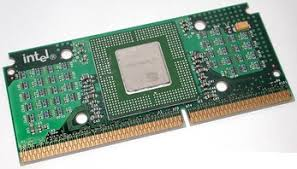
\includegraphics[width=0.5\textwidth]{cache}
\end{figure}
\subsection{Describa la manera como se gestiona la memoria en un computador:}
La memoria en el computador se debe administrar eficientemente, algunos programas necesitan unos campos de memoria para funcionar eficientemente, y cuando ya no se requiere la gestion de memoria libera estos espacios para futuros programas.
Todo este registro lo lleva el administrador de memoria, proporcionando protección y uso compartido, debe facilitar un espacio para cada proceso.[1]
\subsection{Qué hace que una memoria sea más rápida que otra?:}
La velocidad se debe a tres factores importantes: a la velocidad del bus, a la frecuencia de reloj que trabaja el bus de datos, y a la cantidad de bits que se transfieren por este bus. Con el paso del tiempo la tecnologia ha ido mejorando estas características dentro de la arquitectura de los computadores o más específicamente de las placas madre o Main Board.
\subsubsection{Por qué es importante?:}
Es mportante porque la velocidad me esta definiendo la tasa de transferencia de información en bits por segundo, y para que este proceso sea eficiente, las memorias deben ir avanzando según la arquitectura de los computadores actuales, especificamente los buses de datos.


\newpage
\section{Conclusión} \label{conclulsion}

La tecnología esta avanzando a un ritmo exponencial, los sistemas electrónicos han evolucionado cambiando su arquitectura y por ende la memoria como dispositivo importante de los procesos de computo lo hace también, la memoria ha evolucionado, tanto la cache para el procesador, como la Rom y la Ram para permitir procesos más eficientes.
\newpage
\bibliographystyle{IEEEtran}
\bibliography{references}
{Tutorial,
   title = "Learn Computer Fundamentals",
   url  = "https://www.tutorialspoint.com/computer_fundamentals/computer_memory.htm",
   keywords  = "Computer,Fundamentals"
}
\end{document}
